\documentclass[english,a4]{article}
\usepackage[T1]{fontenc}
\usepackage[latin9]{inputenc}
\usepackage{geometry}
\geometry{verbose,tmargin=3cm,bmargin=3cm,lmargin=3cm,rmargin=3cm}
\usepackage{graphicx}
\usepackage{hyperref}
\hypersetup{
    colorlinks,
    citecolor=black,
    filecolor=black,
    linkcolor=black,
    urlcolor=black
}
\usepackage{booktabs}

\usepackage{babel}

\begin{document}

\title{SLOVENIA --- Vodna Sled 2010 --- Interim Report}


\author{James Kirkpatrick, Jana \v{C}arga, Gergely Ambrus and Jarvist Moore
Frost}
\maketitle
\begin{abstract}
\textsc{Vrtnarija: a new 2.2km, all below -500m}

Vodna Sled 2010 was a clear success - in all we discovered 2.2km of
new passage, all below -500m, all in Vrtnarija using \textsc{Camp
X-Ray} (\textsc{Reloaded}, now a plush four bed camp at -550 m) as a base.
The majority of the discoveries lead from a horizontal series near
\textsc{Zimmer} chamber with numerous un-pushed leads for next year
and over 1.5 km of passage. Significant amounts of exploration also
took place in \textsc{Tolminska Korita} concluding with a connection
to the 'deep' level at -653 m, and pushing the \textsc{Republica}
streamway from -744 to -802 m.
\end{abstract}

\tableofcontents

\section{Expedition Overview}

Twenty-two expedition members travelled from the UK for a total of
65 person-weeks in the field, with 88 person-trips in our callout
roster. Seventeen from the UK stayed at underground camp, along with
six Slovenes from the local JSPDT club, a total of 95 people-nights
at camp. All successful exploration took place on camping trips. 
This was the first expedition for three
first-year UK students, all of whom stayed at underground camp and
discovered significant quantities of new cave.

In all, the cave consumed a kilometre of rope for the rerigging of
the main pitch series, and newly explored sections left rigged (or
with rope pulled up) for 2011.

No work during the 2010 expedition went into M2 (Kavkna Jama), directed
towards forging a connection with Vrtnarija. However, during the early
Autumn two JSPDT trips capped through the tight rift at the very end
of the cave (\textasciitilde{}-390m), discovering and then descending
a \textasciitilde{}60m pitch.

The prospects for 2011 are extremely good. The extensive horizontal
development has led to the discovery and initial exploration of a
number of independent streamways and associated pitch series, in a
horizontal slice of the mountain we have never visited.

\begin{center}
%
\begin{figure}
\centering
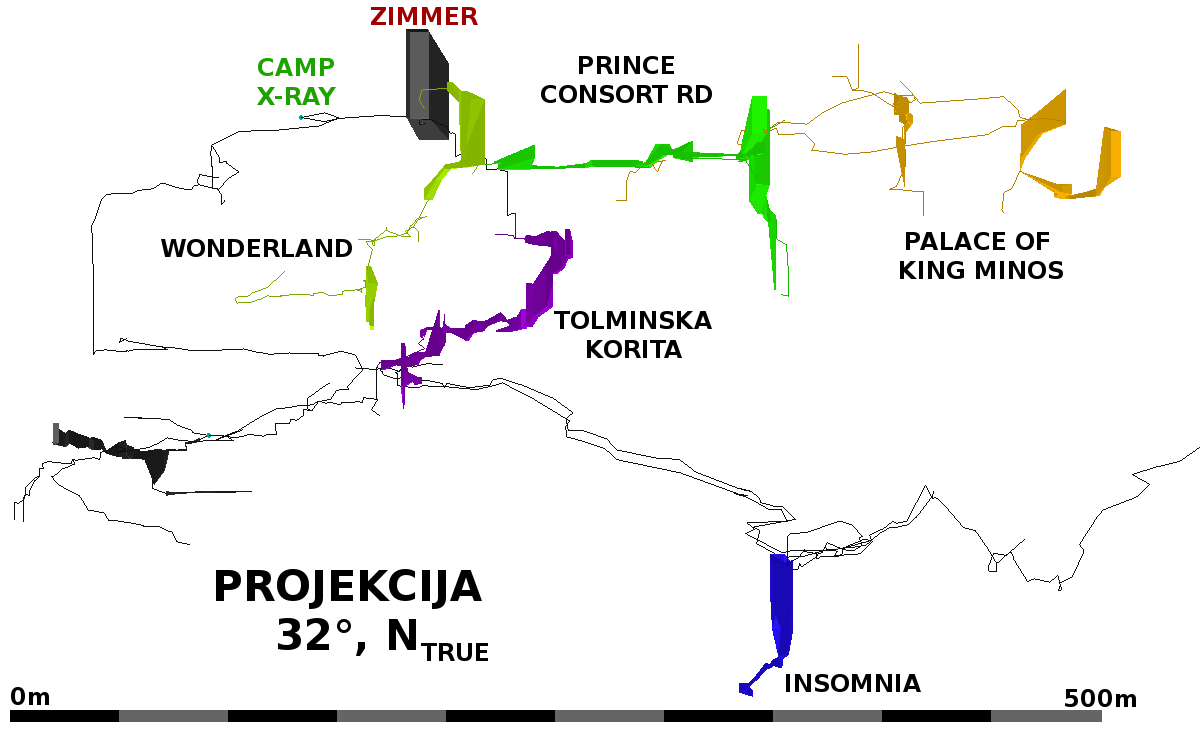
\includegraphics[width=0.85\columnwidth]{2010_deep_vrtnarija_colour_coded_inverted_labelled}

\caption{Colour coded diagram of new cave discovered \& surveyed in 2010 in
Vrtnarija.}



\end{figure}

\par\end{center}


\section{Migovec Background}

The original Migovec discoveries were by the JSPDT in the 1970s (M2,
-350m) and 1980s (M16, -547m). ICCC has been going on regular expeditions
to Migovec since 1994. With the JSPDT this including the finding of
M18 which was connected into M2 and M16 in 1996. This system (SysMig)
was explored to chokes at -937 m and -958 m and sumps at -970 m and
-967 m (the sumps are at 885 m above sea level). SysMig is 11.5 km
in length, most of this length is due to the many vertical shafts
(vertical length of survey is 6.8 km).

The focus of expeditions shifted to Vrtnarija in 2000, which was discovered
and pushed down to -802m by 2004. This cave was initially thought
to be much more linear that SysMig, having a typical vertical entrance
series to -550 m, where a large horizontal phreatic (Friendship Gallery)
led to a pitch (Big Rock) down to an extensive horizontal level. No
true sumps were discovered, the cave was pushed to reach a mud sump
with tiny flow.

During 2005 and 2007 expeditions a small side passage in Vrnarija
(Captain Kangaroo) was pushed. Analysis of the survey data before
summer 2008 suggested that this passage was within 50 m of the M2
part of SysMig, which no one had been down since the 1970s. Connection
of SysMig to Vrtnarija would form the largest alpine system in Slovenia.

During the 2008 expedition, M2 was rerigged. Exploration in Vrtnarija
was concentrated within the 'depth range' of a possible M2 connection
(the best vertical lead, Dark Tranquility, was abandoned at -338 m).
M2, which closes down enormously after -250 m, was slowly pushed with
extension persuasion. 

In 2009, a camp was made in Vrtnarija near the potential connection
to M2. Several climbs and other 'secondary' leads in the vicinity
of camp were probed, without finding the connection. Dark Tranquility
was pushed well below the bottom of M2. This connected to a passage underneath
Friendship Gallery (Falls Road, a small confluence). 
On a trip to rig ropes from Friendship Gallery to allow the physical
connection, an old lead (Korita) was looked at and proved viable.

At the beginning of the 2010 expedition, the known length of Vrtnarija
was 6.575 km.

\begin{center}
\begin{figure}
\centering
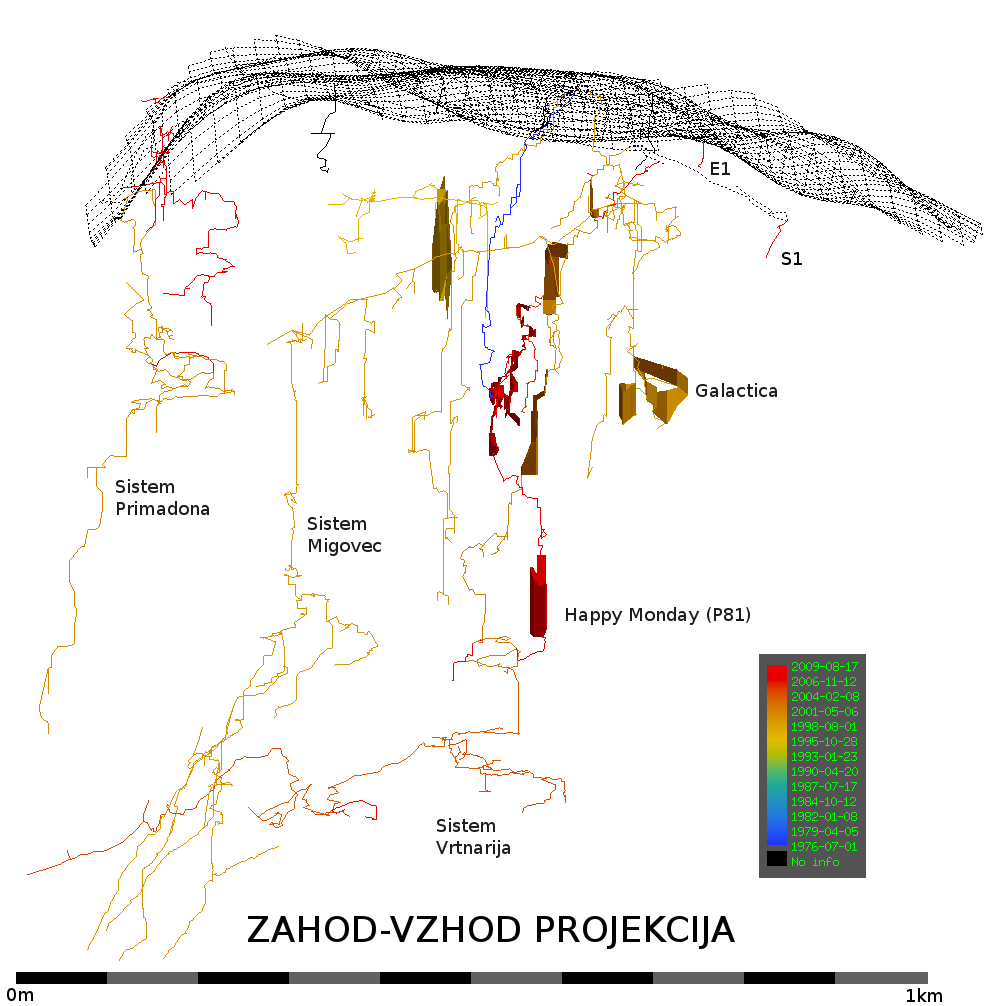
\includegraphics[width=0.75\columnwidth]{mig_2009_for_jamar}
\caption{A West---East projection of the 2009 extent of known cave passage in Migovec, with surface topology
(Digital Elevation Model from Slovene Karst Institute).}
\end{figure}
\end{center}


\section{Expedition logistics}

A nine seater minibus was hired from Imperial College Union for four weeks and two days. 
This was driven
non-stop from South Kensington to Tolmin, Slovenia in just under 24 hours
including the ferry journey (Friday -- Saturday evening). Special permission
had been acquired by the JSPDT to camp in the national park, on top of Migovec
in our usual bivouac spot. The van made two trips to Tolminske Ravne (912 m) on
Sunday morning, where the equipment was unloaded into the barn of the Skalar
family. 

The mountaintop was in continual occupation from Sunday evening, with the first
caving trips on Tuesday.

\subsection{Caving Logistics}

The main route to Friendship Gallery in Vrtnarija contains over 500
m of vertical pitches. Many of these ropes had been in place 
for some time and it was decided to replace them. Six hundred metres of new
ropes were installed in the first few days of caving thanks to concerted
effort, multiple waves of rigging teams and an 'all hands on deck' attitude
from the whole expedition team.  Other factors that aided a quick start to the
exploration were:
\begin{itemize}
\item the significant amounts of dried foods left in loco at the bivouac
site on Migovec (thereby saving on porterage time at the beginning
of expedition); 
\item the sending of an 'advance party' to set up the bivouac and collect
drinking water (a day of back breaking snow haulage) before the main
group arrived; 
\item the fact that all underground camping kit was carefully packed in
transport sacks in England. 
\end{itemize}
These logistical steps meant that within the first week of the main
expedition group arriving in Slovenia most of the porterage had been
done, the cave had been re-rigged and a 4-bed underground camp at
the X-ray (-550m) site had been set up. In fact, the very first survey
data was recorded at -606m exactly seven and a half days after the
van left South Kensington.


\subsection{Expedition Talks}

An expedition slideshow was given by Jarvist Frost, with translation by Jana
\v{C}arga, on the Saturday evening at the end of expedition before departing
for Britain.

An expedition talk was presented by Jarvist Frost at Hidden Earth 2010.

\section{Expedition Findings}

The initial effort of the expedition was directed into setting up underground
camp. As the first pushing trips from this underground camp came back with
positive news, exploration based from camp (i.e. deep in Vrtnarija) quickly
became the main focus of expedition effort. This came at the cost of further
work in bounce trips down Captain Kangaroo (Vrtnarija, the likely connection
region to M2) and M2 / SysMig itself. 

The usual surface bashing continued, looking for new cave systems on the
plateau. A revisit was made to the area north of Kuk. This region is heavily
cratered with clear cave development, but the fear is that the limestone is too
broken and chossy for a human sized entrance. 

We first visited this region with a serious aim of cave exploration in 2008,
and returned in December 2009 on a `winter recce' by a two person team with ice
axe and crampons to identify which surface features were actively linked into
extensive underground systems through the holes blown in the snow. Several more
entrances were identified during this recce, ones that were likely to be
continued to be ignored in the summer due to their unusual position.

These entrances were relocated this summer, but no new descents were made.

\subsection{Leopard --- 1.5km of new passage}

\begin{figure}[!h]
\centering
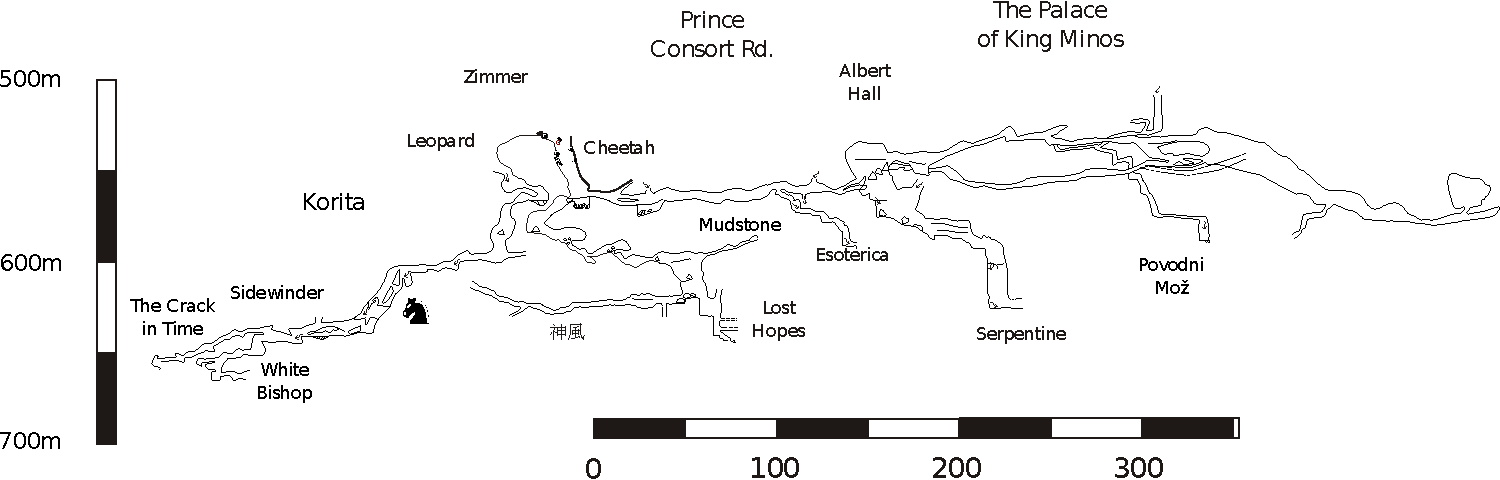
\includegraphics[width=0.9\columnwidth]{2010_new_stuff_extended_extraction}
\caption{Extended elevation of new cave discovered in \textsc{TOLMINSKA KORITA} and \textsc{PRINCE
CONSORT} during 2010 Expedition.}
\end{figure}

Leopard became the great focus of exploration this year. This lead
(a window off Zimmer chamber, now a 15m 'up' pitch) had also been
originally discovered in 2001, but the drop that it led to had lain
untouched since then. 
This was partially due to its loose and muddy nature, but also that deep
exploration had concentrated on good leads elsewhere (most particularly the
lower Vrtnarija level accessed with the bottoming of \textsc{Big Rock}). This
took several sessions of rigging and gardening to successfully conquer, and is
is now named Cheetah (P35m), because of the sense of having cheated death that
it engenders on passing. There are several windows off Cheetah, which are
definitely promising, although not easily accessible because of the broken nature
of the rock.

At the bottom, it intersects a horizontal, fossil passage, which has
been explored in three main horizontal parts:

Wonderland (heading South) linking into Rolling Stones, Surprise,
Mudstone Traverse, Kamikaze and finally Lost Hopes. Mainly dry with large breakdown chambers. 

Prince Consort Road (heading North) was initially pushed to \textsc{The Albert
Hall} (from where the \textsc{Serpentine} meander leads off to the \textsc{It
Will Rain for a Million Years} pitch), bisects three streamways (one of which
was pushed and forms the Esoterica series) and includes considerable calcite
formations.

From \textsc{The Albert Hall} a climb was made into the
\textsc{Palace of King Minos}. This passage is complex, and side branches have neither been fully
explored nor surveyed. The known passage leads via Minotaur Rift to terminate in the
Queens Bed Chamber where the draught disappears towards the ceiling.

Together this passage leading off from Cheetah has been explored to over 1.5 km in length,
and we are sure that more is yet to be found. 

A significant volume of air flows through these regions, indicating that there may
be further developments.

\subsubsection{Wonderland}

Wonderland is the southern-most of the horizontal development, leading
directly off from Cheetah. It was pushed to a small pitch dropping
into a boulder filled chamber, Rolling Stones, which was the limit of the first
exploration trip due to the lack of rope.  This chamber is situated right below
Zimmer, about 40m deeper. There is a further, as yet unpushed, pitch going down
between the large, seemingly unstable, boulders on the floor.

A happen stance crawl behind some boulders led to further drafting
passage (Hidden Surprise), which, after traversing another chamber
and crawl, finishes in a chamber with a massive hole in the floor
(Kamikaze pitch). The passage continues on the far side of the pitch
(traversed on mud along the left wall), however, due to the collapsed
ceiling, these developments are almost two-dimensional (Mudstone Squeeze).
The squeeze, which is filled with interesting fossilised mud formations,
was pushed to the limits of comfort, although it still continues.

Kamikaze consists of a series of small ledges. From the second ledge
a tell tale breeze led to an interesting bedding plane crawl pushed
upwind but still untouched downwind. The pitch was bottomed (Lost
Hopes), wherein an inlet was followed down a 10m pitch to a series
of squeezes and rifts which quickly became tight. There is a ledge
halfway down Lost Hopes, with a perhaps larger abandoned rift.

These three leads (Kamikaze, Mudstone, Lost Hopes) are of interest
as they now form the most Easterly extent of Vrtnarija at depth, seeming
to 'spear' through the large N-S geological feature that contains
the majority of the horizontal passage.

The whole area of Wonderland is extremely dry, quiet and rather spacious
in its scope. It is particularly reminiscent of the higher level passage
in the Easegill system, Yorkshire.


\subsubsection{Prince Consort Road}

Prince Consort Road is the passage going north from Cheetah. Several
streams intersect it and some formations have been found there. The
discovery of stalactites covered with helictites proved particularly
exciting! The passage leads to a small boulder choke which was easily
surpassed and led to a large chamber (the Albert Hall). Before the
Albert Hall, three apparently unique streamways have been found:

One intersecting the passage along a traverse (water chokes into boulder
floor), then around a small chamber at about halfway to Albert Hall,
on a corner of the main massage approximately 2/3 of the way to the
Albert Hall a small rift to the east, and a nice white-sanded water
inlet to the west. The latter leads to an unpushed pitch under the
main passage, there is a cairn and note mentioning the lead. Of these,
only the second has been pushed, into the Esoterica series. Strangely
this wet, tight rift has only been visited once during the expedition,
even though it is still going!

In the Albert Hall two streams enter the chamber from on high (the
ceiling was measured as being over 30m up, by laser disto) and join
into a rather beautiful spacious vadose streamway (The Serpentine).
Serpentine was pushed and leads to another split pitch (It Will Rain
for a Million Years \textemdash{} pushed during a continuing flood
pulse). At the bottom of It Will Rain pitch the stream continues and
has not been explored.

\subsubsection{The Palace of King Minos}

North from the Albert Hall a muddy climb lead to The Palace of King
Minos. This passage and its continuation (The Minotaur Rift) has some
of the most beautiful formations found on Migovec to date, in particular
fine walls of calcite, gypsum and aragonite crystals, mud formations
and weird soot encrusted floors. The Palace has a labyrinthine nature
with several passages leading back to Albert Hall, the largest loop
of which was named Ouroboros

The passage has a classic large phreatic lozenge shape, with some
parts undercut by fossil vadose passage. Near the start of the passage
a significant breeze blew through a small hole. This was enlarged
and found to lead to a small phreatic tube which bizarrely led into
an active vadose streamway (Povodni Mo\v{z} \textemdash{} Water Nymph).
Povodni Mo\v{z} has been pushed upstream to a large active aven (and smaller
dry parallel shaft), and downstream to a sump (approximately 2mx2m
in size in the corner of a small chamber and taking the small flow)
and has hence been derigged.

Continuing along the main Palace passage several horizontal tubes
have been explored which lead back into the main passage, though not
all have been entered in the survey. Eventually the main route leads
to a high and wide rift (Minotaur Rift \textemdash{} 20m high, 60m
long) beyond which the best formations are to be found. This passage
has a few interesting leads in it: a high, dry, circular, muddy window
to the right of the passage near a tiny inlet, 2 small tubes leading
off the main passage which both need a little mechanical persuasion.

The chambers beyond Minotaur Rift are spacious and display massive
amounts of crystal formation on all available surfaces --- there is
white `popcorning' almost everywhere, with regions of more intricate
needle and feather formations. The chambers decay into a crawl, which
almost unbelievably is over a smooth calcite floor. This leads to
a classic boulder choke gallery (choking at the end). On the left
a small boulder choke climb leads to the Queens Bed Chamber. In this
large room, the draught appears to disappear up towards the ceiling
- both ends of the chamber are potential climbing projects (\textasciitilde{}+20m).

The region is extremely reminiscent of Ogof Ffynnon Ddu II in Wales.


\subsection{Tolminska Korita}

This lead of Zimmer chamber had been discovered in 2001 but had lain
unexplored until last year, when the first few pits of the active
meander were pushed to a larger pitch. Korita developed into cascades
of active pitches (Black Knight series) to a duck. The duck was soon
bypassed by a 5m free climb into old phreatic level. 

The passage beyond
soon diverges into two continuations:

\subsubsection{Sidewinder, Crack in Time}

The higher dust filled dry phreatic level (Sidewinder, Crack in Time) connects
into \textsc{Envy} in the low level via free climbs and two small pitches. It
is not particularly surprisingly that the `Crack in Time' was not explored from
below, as the connection is made by a long body-sized crawl above a thin (5 cm)
crack connecting to known passage (Envy), which happily pops out at the top of
a obscure 3 m free climb. Connecting into a 2004 era permanent survey station,
Korita now forms a second loop in Vrtnarija, forming Vrtnarija into a figure-8
shape with Friendship Gallery at the waist.

\subsubsection{White Bishop, Stalemate}

The active streamway descends 
two 10-15 m pitches connected with a spacious meander incorporating free
climbable cascades, before ending in an impassable rift (-662 m). 

This water disappears into `blank mountain' on
our survey, but would require considerable effort to progress, and Korita
was thus derigged.

\subsection{Roaring Floor Tease (Muddy Window off Happy Monday)}

This was regained by bolt climbing from the bottom of Happy Monday to regain the Muddy Window. 
The climb in the mud chamber was made, but quickly led to a large boulder
blocking the way. A tight rift taking a large draught was left unpushed.
Progress is believed to require expansion.

Similarly the traverse to an inlet on Falls Road, and the continuation
of Falls Road itself was left unpushed. A small dig was made in Friendship
gallery beyond Prima junction, which led to a small unpushed pitch
above a stream.

\subsection{Deep Leads (Below \textsc{Big Rock Candy Mountain})}

\subsubsection{Insomnia - Republika Streamway}

Last year a `written off' streamway (Republika, leading from Red Cow)
was found and pushed upstream to an aven fed watershed, then down
the other limb to a rift pitch.

With the promise of being one of the deepest points of the cave a
return in 2010 was obligatory. The pitch was found to be 41m and was
pushed down a continuing active rift (Insomnia). The end is now only
4m higher than Colorado Sump (the deepest known point of Vrtnarija).
Since the limit of exploration is above a small 4-5m pitch it is understood
that in 2011 this will inevitably become the deepest passage in the
system, and the signs are good for continuing development of depth.
The end is 802m below the entrance of Vrtnarija, but the M2 (Kakna
Jama) entrance is 75 m higher still, and a connection between the
systems would make this point -877m deep overall, with potential for
further depth extension.


\subsubsection{Balamory}

A return to Balamory was thwarted by lack of rope of the exploratory
party (one more pitch than expected on route), but the team made good
use of the trip to the depths by recovering the camping mats from
the deep 2004 camp (The Fridge, near Cactus Junction), and prospecting for
other leads with some success.

\subsection{M2 --- Kavkna Jama}

The JSPDT organised a trip based at the mountain hut at Kal on 2nd October
2010. The terminal rift was enlarged to gain a $\approx$ 20 m pitch and a
larger, undescened (due to lack of rope), pitch. 

A return trip three weeks later descended the pitch and found it to be
$\approx$ 60 m. The cave closes immediately, with a tight rift taking the water
and a slightly larger abandoned rift also offering potential. It draughts
strongly.

The M2 cavers returned in thick fog, following their footsteps through the 10
cm deep snow. With the coming winter Migovec is effectively closed for
exploration until summer 2011.

\section{Exploration Outlook}

In all, 2.2km of new cave was found during the 2010 Vodna Sled expedition,
taking Vrtnarija to 8.776 km.

We are in the extremely fortuitous circumstance where we finish the year with
considerably more leads in the Migovec cave systems than we started with.  The Vrtnarija camp
was derigged with the certainty that we will be back next year camping in the
same location. Gas cylinders and cans of fish were left sealed in Daren drums
with a rock of carbide to keep them dry, the carry mats and tents were left
standing to air, and we have a considerable armoury of rope brought back from
the pushing fronts waiting for the 2011 team.

The work by the JSPDT in the Autumn has `opened up` M2 once again and brought
the possibility of forging a connection back to the table. 

The pushing of the Republica streamway (now Insomnia) to within a few metres of
the maximum depth of the cave has reawakened the possibility of further depth
extension to Vrtnarija. Expedition members have mooted the possibility of
establishing an additional 2-man `deep camp' to benefit pushing trips in the
lower reaches of the cave, particularly any revisits to the far North end of
the system.

\subsection{Migovec's Long Term Prospects}

It has been a recurrent discussion in our club as to when we will run out of
new cave to discover in Migovec. Almost all of our fruitful exploration has
taken place within a single square kilometre of the flat topped mountain. 

Migovec, being part of a mountain chain that is the first high altitude
interruption to moist air from the Adriatic, receives an extremely significant
level of rainfall. This summer, Jaka Ortar, a Slovenian geographer, recorded
210cm of rain on Migovec in 100 days (28th July-3th November) with his network
of rain gauges. However we have never found any large rivers underground ---
the known cave can only account for a tiny percentage of the total drainage for
the plateau.

Our current hypothesis is that there is no `master system` gathering the water,
but instead a complex hydrology induced by cave passage intersecting the
underlying (as yet, unvisited) band of Cretaceous shales.

For all Vrtnarija's complexity, the entire cave can be fitted into
a slab of limestone slanted at 66 degrees and just 1000x150x1000m.

Certainly, as long as we can continue to find entrances through the frost
shattered and heavily cratered surface, there will be enough cave in Migovec
for decades more of exploration.

\section{Sponsorship and Thanks}

\begin{itemize}
\item{Ghar Parau Foundation --- Expedition equipment fund (rope!)}
\item{Beast Products --- Sponsorship in Kind (technical fleeces for underground
camp)}
\item{Starless River --- Starless River for a large discount on expo equipment,
and gear advice.}
\item{Imperial College Trust and Imperial College Union --- Tour funding (transport) }
\end{itemize}

\section{Conclusion}

The significant discoveries of this year have been the fruit of the
communal effort of ICCC and JSPDT members. When System Vrtnarija and
System Mig will be connected, the cave will only be 500m shorter than
Postonjska Jama system. Suddenly the plain dwellers will have to rewrite
their tourist brochures and the thought of the longest cave in Slovenia
will not be a dream. Oh, and the cave has the potential to be 1km
deep (requiring an additional 120m of depth from Insomnia).

As well as being proud of each metre of survey we should also think
about each metre that a tackle sack was carried, each meal cooked,
each bottle of booze safely ferried to camp. A significant factor
in our success is evident because it needs not mentioning: thanks
to efficient and thoughtful organization we did not run out of any
goods, the stereo batteries were always full, the food supplies always
high. And most importantly, we have no accidents to report.

\section{Rope Testing}

The rope removed from the main pitch series in Vrtnarija is currently being
drop tested by Bob Mehew on the BCA rope testing rig. This will hopefully
provide some useful information the extent of degradation of SRT ropes used in
Alpine exploration, and the associated `permanent' rigging.

\section{Expedition Photos}

Expedition photos are available on the Imperial College Caving Club website at the following address:\\

\url{http://www.union.ic.ac.uk/caving/photo\_archive/slovenia/2010/}

\section{Surveyed Discoveries}

Current survey data is available for the entire Tolminski Migovec plateau on the Imperial College Caving Club website in Survex format:\\

\url{http://www.union.ic.ac.uk/rcc/caving/slovenia/MigSurveyData/}
\\
An alphabetically sorted list of new discoveries during Vodna Sled 2010 is presented here:\\

\begin{tabular}{l c}
Name & Polygon Length \\
\midrule
Black Knight & 116.08 m \\
Consort & 239.99 m \\
Crack in Time & 44.60 m \\
Esoterica & 63.24 m \\
Insomnia & 100.30 m \\
It Will Rain & 48.92 m \\
Kamikaze & 159.60 m \\
Korita & 86.39 m \\
Lost Hopes & 35.62 m \\
Palace of King Minos & 589.63 m \\
Mudstone & 53.36 m \\
Povodni Moz2 & 161.20 m \\
Povodni Moz & 27.69 m \\
Rolling & 48.27 m \\
Serpentine & 70.53 m \\
Sidewinder & 23.86 m \\
Stalemate & 35.73 m \\
Surprise & 71.24 m \\
White Bishop & 52.86 m \\
Wonderland & 134.29 m \\
\midrule
Total & 2163.40 m \\
\end{tabular}

\subsection{Vrtnarija Loop Closures}

Our survey is now corrected to grid north based on the NOAA American
Webservice, with Lat + Long on M10/Bivi, calculated for 1st Aug of each year.
This was mainly to agree with surface DEM data \& GPS data (declination is
approximately 2.5 degrees), as the rate of change of declination is slow (6
minutes a year).

Vrtnarija possess two large loops, making the cave into a `figure 8' configuration. 

During 2009 the Captain Kangaroo --- main pitch series loop was closed
(consisting of data collected from 2000--2009, approximately 1.8km loop).
During 2010 the Tolminska Korita -- Big Rock loop was closed (data from
2001--2010, approximately 1.7km loop).

All sampled misclosures were 1.5--2.0 \%. Typically the horizontal misclosure
was twice that of the vertical (our total plan length of survey polygon is also
approximately double the total vertical length).


\section{Rainfall Response of Vrtnarija}

Assessing the flood response of the cave is obviously extremely important
with respect to the safety of the expedition members and continued
cave exploration. This year we had several periods of extended, extremely
heavy rain, whilst people were underground and the nature of the pitches
was inspected.

As well as for reasons of safety, due the expected difficulty in acquiring
permission to internally dye trace streams, comparing flow volumes
is the best method we have of understanding the hydrological connections
within our cave.

\subsection{Vrtnarija Main Pitch Series}

\subsubsection{Laurel to Pico}

Laurel gets very drippy during heavy rain (with a small stream entering through
an immature development part way down), but quickly clears after the end of the
storm. This water is followed to the top of Pico (supplemented by a usually dry
inlet below I Scream), but all pitches are rigged dry and fully passable. 
The water disappears below boulders at the top of Pico, and is possibly
regained a short distance into Captain Kangaroo where it forms the mostly
hidden stream in the immature rift which is followed to Bonus Chamber where it
flows into a narrow rift (unpushed) below a boulder choke.

\subsubsection{Pico to Pink}

Pico itself is rigged entirely dry, but an inlet splashes the far side of the
pitch. Again, this water is then followed down Terra, Nova and Swing, but these
are also rigged dry. The water flows into a pool in The Officer's Club, whereas
the main route follows a higher abandoned level. Tessellator and the first hang
of Space Odyssey are entirely dry, a considerable volume of water enters on the
bottom hang of Space Odyssey. The rigging is entirely clear of the
water. This water then disappears down a hole down 'the back of' Concorde.

Concorde itself is then mostly dry, with the last two rebelays being
slightly drippy. Strangely, the volume of drips does not seem to vary
much with rain on the surface. This small volume then flows 
down Alchemy, Zlatorog and Fistful of Tolars (again, entirely separate
from the rope) and is believed to flow into the Banzai streamway.

\subsubsection{Pink to Zimmer}

The first pitch in Pink is dry under normal conditions --- with a considerable
volume of water entering out of a bedding plane in the rock and flowing over
the pitch about \textasciitilde{}5m from the rigged location. However, heavy
rainfall can result in a sheet of water flowing closer to the final hang, and
even reaching it. 

The volume present on the first pitch in Pink seems comparable to the amount
present on Space Odyssey and it is thus hypothesised that the streams are the
same (i.e. there is a wet parallel pitch series). This water then disappears
(into an unpushed streamway, possibly joining into Banzai). The rest of the
Pink series is dry.

The lower hang in Sky Net takes a small stream during continual rain. The
bottom hang of Zimmer and the rebelay is extremely wet during heavy rain
--- the lower half of the chamber is filled with heavy
flying spray. The water from Skynet enters through a cut-back slot and bounces
off a series of ledges arriving at the floor in a chaotic mess. 
There is an additional, larger, volume of water that enters on the far side of
the Zimmer pitch. The region of Zimmer pitch between the Leopard window and Korita
remains dry, and this may offer an alternative, dry, SRT route. 

We currently believe that the water on Zimmer collects under the boulders, then
flows down Korita and is followed all the way to Crack in Time.

Interestingly, during heavy rain, the draught changes direction in
Friendship gallery. The usual direction is from Zimmer into Friendship Gallery.
This reverses and strengthens during storms on the surface.

The first pitch in Pink and Zimmer are rerig targets for 2011. Once
rerigged, Vrtnarija should be fully passable to and from camp, if not pleasant,
in all water conditions.

\subsubsection{Leopard}

The main horizontal passages are entirely dry - except for passing
the first streamway, where a rebelay on the traverse was found to
be under the main flow during a flood pulse! Rerigging with a short
pitch down to the boulder choke pit and another at the far side has
been hypothesised for 2011. All of Wonderland and the Palace of King
minos is dry. The vertical leads following streamways, naturally,
are not.


\subsubsection{Korita}

During a flood pulse all the pitches were found to be passable, except
for the top hang of Black Knight pitch, where the deviation was found
to be submarine. A considerable flow existed in the tight rifts and
so drenched feet were a constant risk.


\subsubsection{Republica}

The region was found to be fairly damp - with falling water in heavy conditions
soaking a rebelay. 

Big Rock is drippy, but entirely passable.


\end{document}


